%! Author = wolfram_e_laube
%! Date = 16.04.24

\item[(c)]
The output signal $y[n]$ is plotted using Python with the following code:

\begin{verbatim}
import matplotlib.pyplot as plt

# Plot the output signal
plt.figure(figsize=(10, 4))
plt.stem(np.arange(Ly), y, basefmt=" ", use_line_collection=True)
plt.title('Output Signal $y[n]$')
plt.xlabel('Sample index $n$')
plt.ylabel('Amplitude')
plt.grid(True)
plt.show()
\end{verbatim}

This script uses the `matplotlib` library to plot the output signal $y[n]$.
The `stem` function is utilized to provide a clear depiction of the discrete nature of the signal.
Settings like `figsize` and `grid` enhance the visual presentation, making the plot easy to read and interpret.

\begin{figure}[h]
\centering
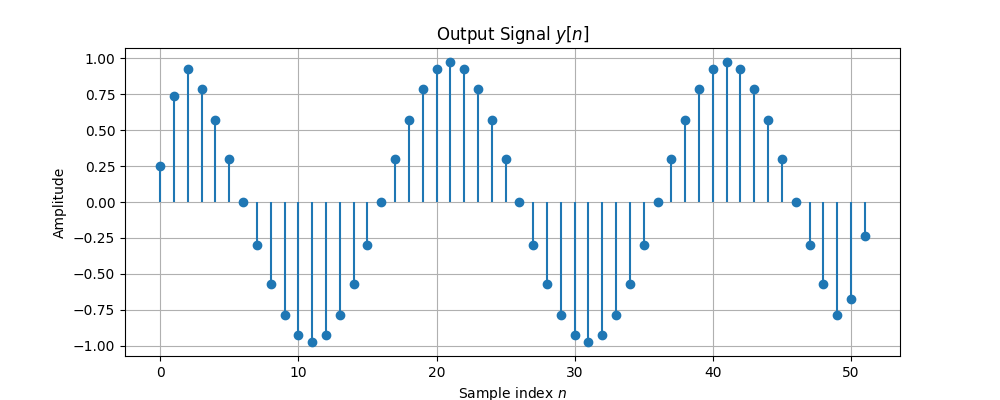
\includegraphics[width=\textwidth]{fig/ex3_plot_1}
\caption{The requested plot}
\label{fig:ex3_plot}
\end{figure}


